\section{Network}

For one neuron there is one output value so we can easily see that one is not enough to solve many problems. Combining neurons into networks and layers will make them more useful. But one single neuron is still able to solve some class of problems.

\begin{wrapfigure}{r}{0.3\textwidth}
    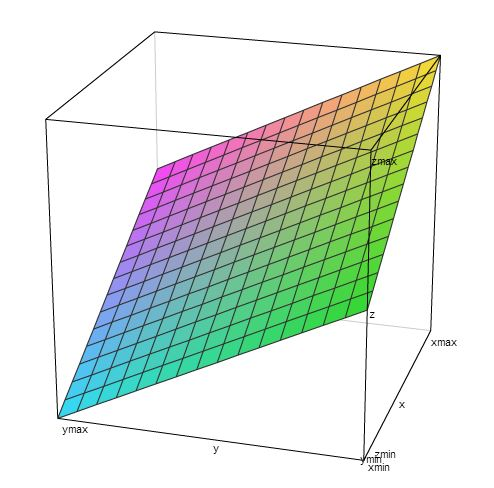
\includegraphics[width=0.32\textwidth]{Media/Plane.png}
    \caption{Single neuron plane}
    \label{fig:SingleNeuronPlane}
\end{wrapfigure}

Typically each neuron has one constant input value. Graphical interpretation of neuron can show why and also what class of problems can be solve with one neuron only.

Consider a neuron with three inputs $n = 3$ and with random weights $w_n$. So we have four axis, three for input data and one to show neuron output. Without one constant input graph of such neuron would be just a random set of points in 4D space.

But if we set one of the inputs constant then we will have only three axis, two for data and one for output value. Because of this one constant input instead of set of random points we will obtain 3D plane (\hyperref[fig:SingleNeuronPlane]{Figure \ref{fig:SingleNeuronPlane}}).

So our single neuron is able to model a $n$D planes. Such plane allows us to distinguish between three possibilities: data are greater then model, smaller or equal. It is enough to solve all linearly separable problems (e.g. logical AND, OR functions). But not all of the problems are linearly separable.


\subsection{Layers}
Before we will solve 

\subsection{MLNN/PLP}

\subsection{Training}